\documentclass[12pt]{article}
\usepackage{latexsym,amssymb,amsmath} % for \Box, \mathbb, split, etc.
% \usepackage[]{showkeys} % shows label names
\usepackage{cite} % sorts citation numbers appropriately
\usepackage{path}
\usepackage{url}
\usepackage{verbatim}
\usepackage{float}
\usepackage{subfig}
\usepackage[pdftex]{graphicx}
\usepackage{hyperref}

\usepackage{xcolor}
\hypersetup{
	colorlinks,
	linkcolor={red!50!black},
	citecolor={blue!50!black},
	urlcolor={blue!80!black}
}


% horizontal margins: 1.0 + 6.5 + 1.0 = 8.5
\setlength{\oddsidemargin}{0.0in}
\setlength{\textwidth}{6.5in}
% vertical margins: 1.0 + 9.0 + 1.0 = 11.0
\setlength{\topmargin}{0.0in}
\setlength{\headheight}{12pt}
\setlength{\headsep}{13pt}
\setlength{\textheight}{625pt}
\setlength{\footskip}{24pt}

\renewcommand{\textfraction}{0.10}
\renewcommand{\topfraction}{0.85}
\renewcommand{\bottomfraction}{0.85}
\renewcommand{\floatpagefraction}{0.90}

\makeatletter
\setlength{\arraycolsep}{2\p@} % make spaces around "=" in eqnarray smaller
\makeatother

% change equation, table, figure numbers to be counted inside a section:
\numberwithin{equation}{section}
\numberwithin{table}{section}
\numberwithin{figure}{section}

% begin of personal macros
\newcommand{\half}{{\textstyle \frac{1}{2}}}
\newcommand{\eps}{\varepsilon}
\newcommand{\myth}{\vartheta}
\newcommand{\myphi}{\varphi}

\newcommand{\IN}{\mathbb{N}}
\newcommand{\IZ}{\mathbb{Z}}
\newcommand{\IQ}{\mathbb{Q}}
\newcommand{\IR}{\mathbb{R}}
\newcommand{\IC}{\mathbb{C}}
\newcommand{\Real}[1]{\mathrm{Re}\left({#1}\right)}
\newcommand{\Imag}[1]{\mathrm{Im}\left({#1}\right)}

\newcommand{\norm}[2]{\|{#1}\|_{{}_{#2}}}
\newcommand{\abs}[1]{\left|{#1}\right|}
\newcommand{\ip}[2]{\left\langle {#1}, {#2} \right\rangle}
\newcommand{\der}[2]{\frac{\partial {#1}}{\partial {#2}}}
\newcommand{\dder}[2]{\frac{\partial^2 {#1}}{\partial {#2}^2}}

\newcommand{\nn}{\mathbf{n}}
\newcommand{\xx}{\mathbf{x}}
\newcommand{\uu}{\mathbf{u}}

\newcommand{\junk}[1]{{}}

% set two lengths for the includegraphics commands used to import the plots:
\newlength{\fwtwo} \setlength{\fwtwo}{0.45\textwidth}
% end of personal macros

\begin{document}
\DeclareGraphicsExtensions{.jpg}

\begin{center}
%\textbf{\Large Crop/Weed Classification in (CWFID) Image Dataset using some Machine Learning techniques through image representation in Bag-of-visual-words (BOW), Vector of Locally Aggregated Descriptors (VLAD) and Fisher Vector (FV)\newline\newline(Machine Learning Final Project)} \\[6pt]

\textbf{\Large Machine learning techniques for Crop/Weed classification in (CWFID) image dataset \newline\newline(Machine Learning Final Project)} \\[6pt]

%\textbf{\Large Crop rows segmentation in sugarcane fields through computer vision techniques \newline \newline  Pattern Recognition Final Project} \\[6pt]
  Fabio Andres Herrera \\[6pt]
  Escuela de Ingeniería de Sistemas y Computación\\
  Universidad del Valle, Cali - Colombia  \\[6pt]
  fabio.herrera@correounivalle.edu.co
  %, \url{www.math.umbc.edu/~gobbert}
\end{center}

\begin{abstract}
\noindent	
This report presents a simple academic exercise which uses Bag-of-visual-words model (BOW), VLAD image representation and Fisher Vector encoding with some machine learning techniques applied for image classification in Crop/Weed Field Image Dataset (CWFID) of top-down looking images of row cultures (organic carrots). A  mean accuracy on the given test data and labels is used as an evaluation metric to allow comparison of different algorithms used for crop /weed classification.

%. The Crop /Weed Field Image Dataset (CWFID) comprises 60 images with annotations with a ground truth vegetation segmentation mask and manual annotation of the plant type (crop vs. weed)

\end{abstract}

\subparagraph{\textit{Key words.}}\textit{Computer Vision, Machine Learning, Phenotyping, Precision Agriculture}

%https://www.cs.princeton.edu/courses/archive/spr08/cos511/scribe_notes/0204.pdf

\section{Introduction}

Machine learning is the science of getting computers to act without being explicitly programmed\cite{5392560}. Machine learning is about learning to do better in the future based on what was experienced in the past. The process of learning begins with observations or data, such as examples, direct experience, or instruction, in order to look for patterns in data and make better decisions in the future based on the examples that we provide. Machine learning is a core subarea of artificial intelligence. Machine learning algorithms are often categorized as supervised or unsupervised \cite{Ratsch2004}.

\begin{itemize}
	\item \textbf{Supervised machine learning :}
	can apply what has been learned in the past to new data using labeled examples to predict future events. Starting from the analysis of a known training dataset, the learning algorithm produces an inferred function to make predictions about the output values. The system is able to provide targets for any new input after sufficient training. The learning algorithm can also compare its output with the correct, intended output and find errors in order to modify the model accordingly.
	
	\item \textbf{Unsupervised machine learning :}
	are used when the information used to train is neither classified nor labeled. Unsupervised learning studies how systems can infer a function to describe a hidden structure from unlabeled data. The system doesn’t figure out the right output, but it explores the data and can draw inferences from datasets to describe hidden structures from unlabeled data.
	
	\item \textbf{Semi-supervised machine learning :}
	fall somewhere in between supervised and unsupervised learning, since they use both labeled and unlabeled data for training – typically a small amount of labeled data and a large amount of unlabeled data. The systems that use this method are able to considerably improve learning accuracy. Usually, semi-supervised learning is chosen when the acquired labeled data requires skilled and relevant resources in order to train it / learn from it. Otherwise, acquiring unlabeled data generally doesn’t require additional resources.
	
	\item \textbf{Reinforcement machine learning :}
	is a learning method that interacts with its environment by producing actions and discovers errors or rewards. Trial and error search and delayed reward are the most relevant characteristics of reinforcement learning. This method allows machines and software agents to automatically determine the ideal behavior within a specific context in order to maximize its performance. Simple reward feedback is required for the agent to learn which action is best; this is known as the reinforcement signal.
	
	
\end{itemize}

\noindent
Machine learning enables analysis of massive quantities of data. The emphasis of machine learning is on automatic methods. In other words, the goal is to devise learning algorithms that do the learning automatically without human intervention or assistance. There are many examples of machine learning problems. Here are several examples:


\begin{itemize}
	\item \textbf{Optical character recognition:} categorize images of handwritten characters 
	\item \textbf{Face detection:} find faces or indicate if a face is present in images 
	\item \textbf{Spam filtering:} identify email messages as spam or non-spam
	\item \textbf{Topic spotting:} categorize news articles
	\item \textbf{Medical diagnosis:} diagnose a patient as a sufferer or non-sufferer of some disease
	\item \textbf{Customer segmentation:} predict which customers will respond to a promotion
	\item \textbf{Fraud detection:} identify credit card transactions which may be fraudulent
	\item \textbf{Weather prediction:} predict, for instance, whether or not it will rain tomorrow
\end{itemize}


The entire process of a typical learning problem is depicted in Figure \ref{figure4}.
\begin{figure}[H] \centering
	\caption{Diagram of a typical learning problem. }
	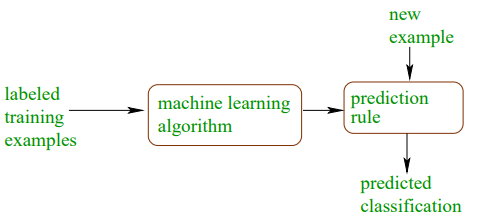
\includegraphics[width=0.6\textwidth]{image4.png}
	\label{figure4}
\end{figure}





There are literally thousands of learning algorithms available. The key to not getting lost in this huge space is to realize that it consists of combinations of just three components \cite{Domingos2012}. The components are:

\begin{itemize}

\item \textbf{Representation:} A classifier must be represented in some formal language that the computer can handle. This set is called the hypothesis space of the learner. If a classifier is not in the hypothesis space, it cannot be learned. 

\item \textbf{Evaluation:} An evaluation function (also called objective function or scoring function) is needed to distinguish good classifiers from bad ones.The evaluation function used internally by the algorithm may differ from the external one that the classifier want to optimize.

\item \textbf{Optimization:} A method to search among the classifiers in the language for the highest-scoring one. The choice of optimization technique is key to the efficiency of the learner, and also helps determine the classifier produced if the evaluation function has more than one optimum.
\end{itemize}


\subsection{Image Dataset}

The dataset comprises field images in top-down view that were acquired with the autonomous field robot Bonirob\cite{BOSH} in an organic carrot farm in 2013. The images were captured while the crop was in growth stages where one or more true leaves were present. All images are annotated and a ground truth vegetation segmentation mask is available together with crop/weed annotations. Figure \ref{figure1} shows a field image (a), a segmentation mask (b) and Crop/weed annotation image (c) even a file in YAML format with a list of polygon vertices and labels.

\begin{figure}[H] \centering
	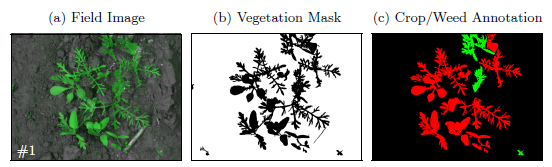
\includegraphics[width=1\textwidth]{image1.png}
	\caption{Sample images from the dataset (a) with ground truth vegetation masks
		and crop /weed annotations. The annotation images (b) and (c) are supplied for
		every image of the dataset. Modified from \cite{Haug2015}. }
	\label{figure1}
\end{figure}


\noindent
The dataset images ware acquired by a JAI multi-spectral camera that captures both visible and near-infrared light was used and mounted on the robot. The camera was looking downwards and the area under the robot was shaded and artificially lit to avoid changing lighting conditions. Figure \ref{figure2} describes the camera setup and its configuration.

\begin{figure}[H] \centering
	\caption{Description of camera system and acquisition parameters. Modified from \cite{Haug2015}. }
	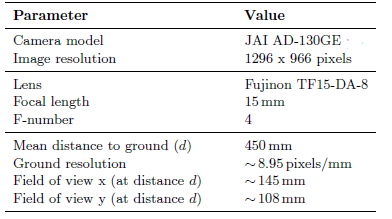
\includegraphics[width=0.6\textwidth]{image2.png}
	\label{figure2}
\end{figure}

\noindent
The Crop /Weed Field Image Dataset (CWFID) was downloaded from:
\begin{itemize}
	\item {\textbf{CWFID Image Dataset:} } \url{http://github.com/cwfid}
	
\end{itemize}

\noindent
The following Jupyter Notebook file shows how the files were read 

\begin{itemize}
	\item {\textbf{Reading Crop and Weed Dataset:} } \url{https://github.com/AndresHerrera/Proyecto_MachineLearning/blob/master/JupyterNotebook/ReadCropWeedDataset.ipynb}
	
\end{itemize}

\section{SIFT Descriptors} \label{sift}
The scale-invariant feature transform (SIFT) is an algorithm in computer vision to detect and describe local features in images. A SIFT descriptor is a 3-D spatial histogram of the image gradients in characterizing the appearance of a keypoint. The gradient at each pixel is regarded as a sample of a three-dimensional elementary feature vector, formed by the pixel location and the gradient orientation. Samples are weighed by the gradient norm and accumulated in a 3-D histogram h, which (up to normalization and clamping) forms the SIFT descriptor of the region. An additional Gaussian weighting function is applied to give less importance to gradients farther away from the keypoint center. Orientations are quantized into eight bins and the spatial coordinates into four each, as seen in Figure \ref{figure6}:

\begin{figure}[H] \centering
	\caption{The SIFT descriptor is a spatial histogram of the image gradient \cite{sift}. }
	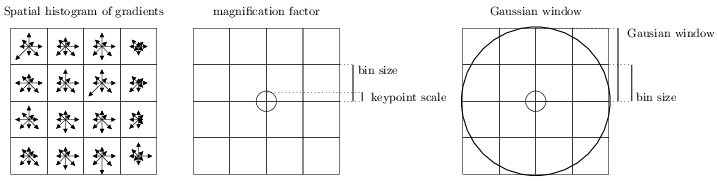
\includegraphics[width=1\textwidth]{image6.png}
	\label{figure6}
\end{figure}



\section{Bag of Visual Words (BovW)} \label{bow}

To represent an image using the BoW model, an image can be treated as a document. Similarly, "words" in images need to be defined too. To achieve this, it usually includes following three steps: \textbf{feature detection}, \textbf{feature description}, and \textbf{codebook generation}. A definition of the BoW model can be the "histogram representation based on independent features".

\begin{itemize}

\item \textbf{Feature representation} After feature detection, each image is abstracted by several local patches. Feature representation methods deal with how to represent the patches as numerical vectors. These vectors are called feature descriptors. A good descriptor should have the ability to handle intensity, rotation, scale and affine variations to some extent. One of the most famous descriptors is Scale-invariant feature transform (SIFT). SIFT converts each patch to 128-dimensional vector. After this step, each image is a collection of vectors of the same dimension (128 for SIFT), where the order of different vectors is of no importance.

\item \textbf{Codebook generation} The final step for the BoW model is to convert vector-represented patches to "codewords" (analogous to words in text documents), which also produces a "codebook" (analogy to a word dictionary). A codeword can be considered as a representative of several similar patches. One simple method is performing k-means clustering over all the vectors.Codewords are then defined as the centers of the learned clusters. The number of the clusters is the codebook size (analogous to the size of the word dictionary).

\end{itemize}

Thus, each patch in an image is mapped to a certain codeword through the clustering process and the image can be represented by the histogram of the codewords.









\section{VLAD} \label{vlad}

VLAD is constructed as follows: regions are extracted from an image using an affine invariant detector, and described using the 128-D SIFT descriptor. Each descriptor is then assigned to the closest cluster of a vocabulary of size $k$ (where $k$ is typically 64 or 256, so that clusters are quite coarse). For each of the k clusters, the residuals (vector differences between descriptors and cluster centers) are accumulated, and the $k$ 128-D sums of residuals are concatenated into a single $k$ × 128 dimensional descriptor \cite{Arandjelovic2013}.The vector of locally aggregated descriptors (VLAD) is an encoding technique that produces a fixed-length vector representation $v$ from a set $X = {x1, . . . , xn}$ of n local d-dimensional descriptors, e.g., SIFTs, extracted from a given image \cite{Delhumeau2013}.

\section{Fisher Vector} \label{fv}

\cite{Sanchez2013}


\section{Classification Algorithms} \label{classalgs}

\subsection{k-Nearest Neighbor Classification} \label{knn}
The simplest method is the k-Nearest Neighbor classifier. Here the k points of the training data closest to the test point are found, and a label is given to the test point by a majority vote between the k points. This method is highly intuitive and attains – given its simplicity – remarkably low classification errors, but it is computationally expensive and requires a large memory to store the training data.

%\subsection{Linear Discriminant Analysis} \label{lda}
%computes a hyperplane in the input space that minimizes the within-class variance and maximizes the between class distance. It can be efficiently computed in the linear case even with large data sets. However, often a linear separation is not sufficient. Nonlinear extensions by using kernels exist, however, making it difficult to apply it to problems with large training sets.

%\subsection{Decision Trees} \label{dectree}
%These algorithms solve the classification problem by repeatedly partitioning the in put space, so as to build a tree whose nodes are as pure as possible (that is, they contain points of a single class). Classification of a
%new test point is achieved by moving from top to bottom along the branches of the tree, starting from the root node, until a terminal node is reached. Decision trees are simple yet effective classification schemes for small datasets. The computational complexity scales unfavorably with the number of dimensions of the data. Large datasets tend to result in complicated trees, which in turn require a large memory for storage. 

\subsection{Random Forest} \label{randomf}

Random forests is an ensemble model which means that it uses the results from many different models to calculate a response. In most cases the result from an ensemble model will be better than the result from any one of the individual models. In the case of random forests, several decision trees are created (grown) and the response is calculated based on the outcome of all of the decision trees \cite{Horning2010}.   A random forest multi-way classifier consists of a number of trees, with each tree grown using some form of randomization. The leaf nodes of each tree are labeled by estimates of the posterior distribution over the image classes. Each internal node contains a test that best splits the space of data to be classified. An image is classified by sending it down every tree and aggregating the reached leaf distributions. Randomness can be injected at two points during training: in subsampling the training data so that each tree is grown using a different subset; and in selecting the node tests \cite{Bosch2007}.



\subsection{Neural Networks} \label{neuralnetwork}

Neural networks are a computational model inspired by the connectivity of neurons in animate nervous systems.
A further boost to their popularity came with the proof that they can approximate any function mapping via the Universal Approximation Theorem. 

\begin{figure}[H] \centering
	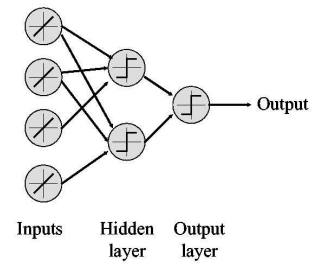
\includegraphics[width=0.4\textwidth]{image5.png}
	\caption{A schematic diagram of a neural network. Each circle in the hidden and output layer is a computational element known as a neuron. }
	\label{figure5}
\end{figure}


A simple scheme for a neural network is shown in Figure \ref{figure5}. Each circle denotes a computational element referred to as a neuron, which computes a weighted sum of its inputs, and possibly performs a nonlinear function on this sum. If certain classes of nonlinear functions are used, the function computed by the network can approximate any function (specifically a mapping from the training patterns to the training targets), provided enough neurons exist in the network and enough training examples are provided.



\section{Comparison} \label{Comparison}


\begin{figure}[H] \centering
	\caption{comparison of machine learning classifiers over different image descriptors. }
	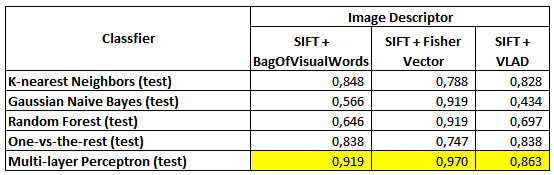
\includegraphics[width=1\textwidth]{class.png}
	\label{class}
\end{figure}


\section{Confusion Matrix} \label{cmatrix}

\subsection{BagOfVisualWords}

\begin{figure}[H] \centering
	\caption{Confusion matrix for K-nearest neighbors classifier. }
	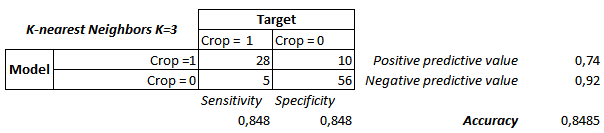
\includegraphics[width=1\textwidth]{m1.png}
	\label{m1}
\end{figure}

\begin{figure}[H] \centering
	\caption{Confusion matrix for Multi-layer Perceptron classifier. }
	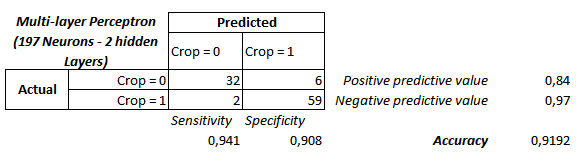
\includegraphics[width=1\textwidth]{m2.png}
	\label{m2}
\end{figure}

\begin{figure}[H] \centering
	\caption{Confusion matrix for Gaussian Naive Bayes classifier. }
	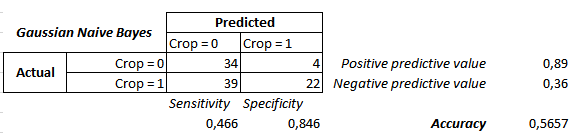
\includegraphics[width=1\textwidth]{m3.png}
	\label{m3}
\end{figure}

\begin{figure}[H] \centering
	\caption{Confusion matrix for One-vs-the-rest classifier. }
	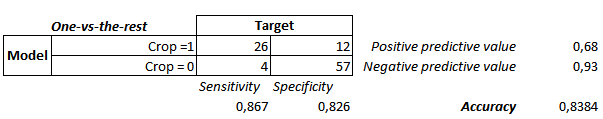
\includegraphics[width=1\textwidth]{m4.png}
	\label{m4}
\end{figure}

\begin{figure}[H] \centering
	\caption{Confusion matrix for Random Forest classifier. }
	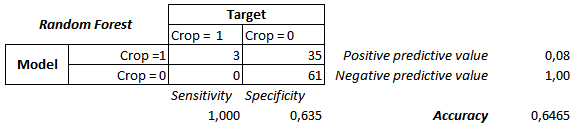
\includegraphics[width=1\textwidth]{m5.png}
	\label{m5}
\end{figure}

\subsection{Fisher Vector}

\begin{figure}[H] \centering
	\caption{Confusion matrix for K-nearest neighbors classifier. }
	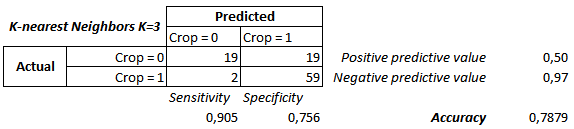
\includegraphics[width=1\textwidth]{m6.png}
	\label{m6}
\end{figure}

\begin{figure}[H] \centering
	\caption{Confusion matrix for Multi-layer Perceptron classifier. }
	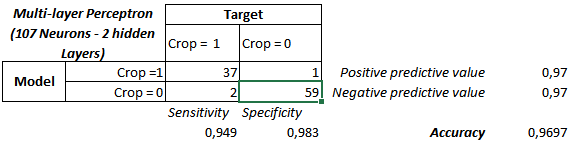
\includegraphics[width=1\textwidth]{m7.png}
	\label{m7}
\end{figure}

\begin{figure}[H] \centering
	\caption{Confusion matrix for Gaussian Naive Bayes classifier. }
	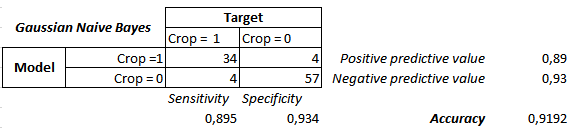
\includegraphics[width=1\textwidth]{m8.png}
	\label{m8}
\end{figure}

\begin{figure}[H] \centering
	\caption{Confusion matrix for One-vs-the-rest classifier. }
	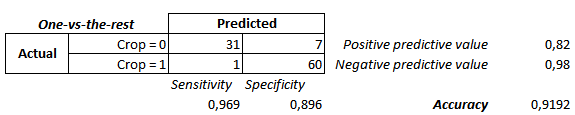
\includegraphics[width=1\textwidth]{m9.png}
	\label{m9}
\end{figure}

\begin{figure}[H] \centering
	\caption{Confusion matrix for Random Forest classifier. }
	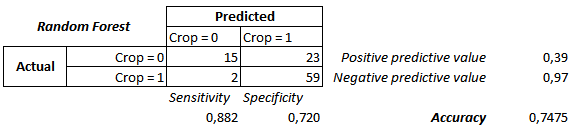
\includegraphics[width=1\textwidth]{m10.png}
	\label{m10}
\end{figure}


\subsection{VLAD}

\begin{figure}[H] \centering
	\caption{Confusion matrix for K-nearest neighbors classifier. }
	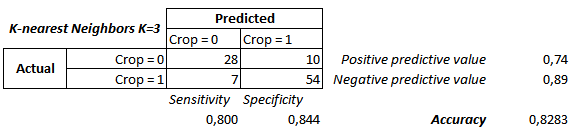
\includegraphics[width=1\textwidth]{m11.png}
	\label{m11}
\end{figure}

\begin{figure}[H] \centering
	\caption{Confusion matrix for Multi-layer Perceptron classifier. }
	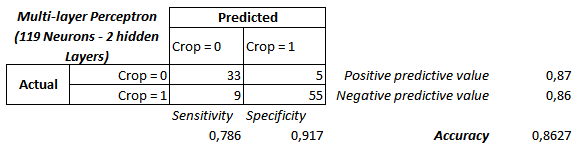
\includegraphics[width=1\textwidth]{m12.png}
	\label{m12}
\end{figure}

\begin{figure}[H] \centering
	\caption{Confusion matrix for Gaussian Naive Bayes classifier. }
	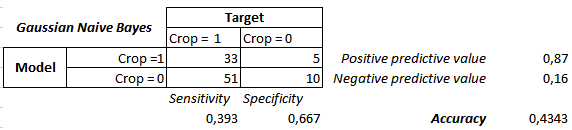
\includegraphics[width=1\textwidth]{m13.png}
	\label{m13}
\end{figure}

\begin{figure}[H] \centering
	\caption{Confusion matrix for One-vs-the-rest classifier. }
	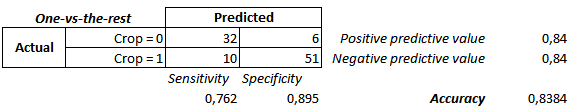
\includegraphics[width=1\textwidth]{m14.png}
	\label{m14}
\end{figure}

\begin{figure}[H] \centering
	\caption{Confusion matrix for Random Forest classifier. }
	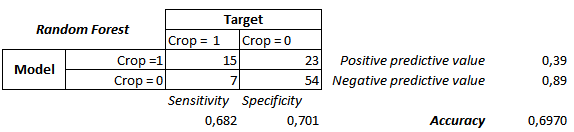
\includegraphics[width=1\textwidth]{m15.png}
	\label{m15}
\end{figure}




\section{Source Code Repository}

Python code blocks and running results are available on GitHub over Jupyter Notebook

\subsection{K-nearest Neighbors Classifier }

\begin{itemize}
	\item {\textbf{BagOfVisualWords - KN :} } \url{https://github.com/AndresHerrera/Proyecto_MachineLearning/blob/master/JupyterNotebook/BagOfVisualWords_KN.ipynb}
	
	\item {\textbf{Fisher Vector - KN :} } \url{	https://github.com/AndresHerrera/Proyecto_MachineLearning/blob/master/JupyterNotebook/FisherVector_KN.ipynb}
	
	\item {\textbf{VLAD - KN :} } \url{	https://github.com/AndresHerrera/Proyecto_MachineLearning/blob/master/JupyterNotebook/VLAD_KN.ipynb}
		
\end{itemize}

\subsection{Gaussian Naive Bayes Classifier }

\begin{itemize}
	\item {\textbf{BagOfVisualWords - NB :} } \url{https://github.com/AndresHerrera/Proyecto_MachineLearning/blob/master/JupyterNotebook/BagOfVisualWords_NB.ipynb}
	
	\item {\textbf{Fisher Vector - NB :} } \url{	https://github.com/AndresHerrera/Proyecto_MachineLearning/blob/master/JupyterNotebook/FisherVector_NB.ipynb}
	
	\item {\textbf{VLAD - NB :} } \url{	https://github.com/AndresHerrera/Proyecto_MachineLearning/blob/master/JupyterNotebook/VLAD_NB.ipynb}
	
\end{itemize}

\subsection{Random Forest Classifier }

\begin{itemize}
	\item {\textbf{BagOfVisualWords - RF :} } \url{https://github.com/AndresHerrera/Proyecto_MachineLearning/blob/master/JupyterNotebook/BagOfVisualWords_RF.ipynb}
	
	\item {\textbf{Fisher Vector - RF :} } \url{	https://github.com/AndresHerrera/Proyecto_MachineLearning/blob/master/JupyterNotebook/FisherVector_RF.ipynb}
	
	\item {\textbf{VLAD - RF :} } \url{	https://github.com/AndresHerrera/Proyecto_MachineLearning/blob/master/JupyterNotebook/VLAD_RF.ipynb}
	
\end{itemize}


\subsection{One-vs-the-rest Classifier }

\begin{itemize}
	\item {\textbf{BagOfVisualWords - OVR :} } \url{https://github.com/AndresHerrera/Proyecto_MachineLearning/blob/master/JupyterNotebook/BagOfVisualWords_OVR.ipynb}
	
	\item {\textbf{Fisher Vector - OVR :} } \url{	https://github.com/AndresHerrera/Proyecto_MachineLearning/blob/master/JupyterNotebook/FisherVector_OVR.ipynb}
	
	\item {\textbf{VLAD - OVR :} } \url{	https://github.com/AndresHerrera/Proyecto_MachineLearning/blob/master/JupyterNotebook/VLAD_OVR.ipynb}
	
\end{itemize}


\subsection{Multi-layer Perceptron Classifier }

\begin{itemize}
	\item {\textbf{BagOfVisualWords - MLP :} } \url{https://github.com/AndresHerrera/Proyecto_MachineLearning/blob/master/JupyterNotebook/BagOfVisualWords_MLP.ipynb}
	
	\item {\textbf{Fisher Vector - MLP :} } \url{	https://github.com/AndresHerrera/Proyecto_MachineLearning/blob/master/JupyterNotebook/FisherVector_MLP.ipynb}
	
	\item {\textbf{VLAD - MLP :} } \url{	https://github.com/AndresHerrera/Proyecto_MachineLearning/blob/master/JupyterNotebook/VLAD_MLP.ipynb}
	
\end{itemize}






\subsection{Jupyter Notebooks}
\begin{itemize}
	\item {\textbf{All Jupyter NoteBook files on GitHub:} } \url{https://github.com/AndresHerrera/Proyecto_MachineLearning/tree/master/JupyterNotebook} 
\end{itemize}

	
	
	





\section{Conclusions}








\section*{Acknowledgments}

To Maria Trujillo Ph.D., a teacher in the course Fundamentals of Multimedia Machine Learning for its valuable training along the fall term 2017.
 

\bibliographystyle{siam}
\bibliography{template}

\end{document}

